\documentclass[titlepage]{article}
\usepackage{fancyhdr}
\usepackage{xcolor}
\usepackage{graphicx}
\usepackage[T1]{fontenc}
\usepackage[utf8]{inputenc}
\usepackage{geometry}
\geometry{a4paper, margin=1.5in}


\pagecolor{white}

\setlength{\headheight}{15pt}
\pagestyle{fancy}
\fancyhf{}
\rhead{Nima Saeidi}
\lhead{Final Assignment}
\cfoot{Page \thepage}


\title{\textbf{Computer Workshop\\ Final Assignment}}
\author{Nima Saeidi \\ student code: 401471318}
\vspace{1in}
\date{6 bahman 1402}

\begin{document}

\maketitle
\tableofcontents

\newpage

\section{Git and Github}
\subsection{Repository Initialization and Commits}
First go Github website. Go to your repository, next using the new button create a new repository. Next you can name your repository and add a readme if you need to and then create the repository. Now you can clone the repository to your computer. Next we create the tex file and add the Github workflow file that was given.

\subsection{GitHub Actions for LaTeX Compilation}
First we need to add .github/workflow file that was given in the example repository to our project. After that you need to also add tags in \textbf{"v*.*.*"} format to your commits then GitHub actions will automatically compile the latex file. The main point is to include the main.yml and its content to your repository.


\section{Exploration Tasks}
\subsection{Vim Advanced Features}
\subsubsection{Folding}
Vim allows you to collapse sections of code or text to make navigation easier. You can fold and unfold sections based on indentation, syntax, or manually define folds. Here's how to use folding:

\begin{itemize}
\item To enable folding, use the command \textbf{":set foldmethod=<method>"}, where \textbf{<method>} can be \textbf{"indent"} for folding based on indentation, \textbf{"syntax"} for folding based on syntax highlighting, or \textbf{"manual"} for manual folding.
\item To fold sections manually, move the cursor to the line you want to fold and use the command \textbf{"zf<movement>"}, where \textbf{<movement>} is a motion command like \textbf{j}, \textbf{k,} \textbf{\}}, etc.
\item To unfold a fold, move the cursor to the folded line and use the command \textbf{"zo"}.
\item To close all folds, use the command \textbf{"zM"}, and to open all folds, use \textbf{"zR"}.
\end{itemize}

\subsubsection{Vimdiff}
Vim comes with a built-in tool for file comparison called Vimdiff. It allows you to view the differences between two or three files and merge changes interactively. Here's how to use Vimdiff:

\begin{itemize}
\item Run \textbf{"vimdiff file1 file2"} to open two files in Vimdiff.
\item You'll see the differences highlighted in colors.
\item Use commands like \textbf{"do"} to obtain changes from the other window, \textbf{"dp"} to put changes into the other window, and\textbf{ "]c"} and \textbf{"[c"} to navigate between changes.
\item After resolving conflicts, save the merged file with \textbf{":w"}.
\end{itemize}

\subsubsection{Registers}
Vim has a feature called registers which allows you to save and recall text, commands, or macros. Registers are like a clipboard where you can store and retrieve content. Here's how to use registers:

\begin{itemize}
\item To yank (copy) text into a register, use \textbf{"ay <movement>} ,where \textbf{"a} is the register name (a-z) and \textbf{<movement>} is the motion command to specify the text you want to yank.
\item To paste from a register, use \textbf{"ap} where \textbf{"a} is the register name.
\item You can also use registers to store macros. After recording a macro with \textbf{q <letter>}, you can yank it into a register with \textbf{"ay} and then paste it later with \textbf{"ap}.
\item Vim also has special registers like \textbf{"*} for the system clipboard and \textbf{"+} for the unnamed register which is used for normal yank and delete operations.
\end{itemize}

\subsection{Memory Profiling}
\subsubsection{Memory Leak}

Memory leaks occur when a program allocates memory but fails to release it when it's no longer needed. This results in wasted memory that cannot be reclaimed by the system, eventually leading to performance issues or program crashes. Memory leaks often happen due to programming errors such as forgetting to deallocate memory, losing references to allocated memory, or improperly managing memory in dynamic data structures like linked lists or trees.

\subsubsection{Memory Profilers}
Valgrind is a versatile programming tool suite primarily used for debugging and profiling applications on Unix-like systems. Its key feature is detecting memory leaks, a common issue where we discussed above, leading to performance degradation or crashes. Valgrind tracks memory allocations and deallocations, providing detailed reports pinpointing the locations of memory leaks in the code. Additionally, it offers tools for detecting memory errors, thread errors, and profiling performance, making it an essential resource for developers working on C, C++, and similar languages to ensure the reliability and efficiency of their software.

\subsection{GNU/Linux Bash Scripting}
\subsubsection{fzf}
\begin{itemize}
\item Fuzzy searching is a technique used in search algorithms to find approximate matches for a given pattern or query string. Unlike exact string matching, where the characters must match exactly, fuzzy searching allows for variations in the characters, such as misspellings, typos, or slight variations in the order of characters. This enables users to search for items even when they are not sure of the exact spelling or when there are minor discrepancies between the search term and the target text.

\item  The command \textbf{ls | fzf } lists the files and directories in the current directory and allows you to interactively select one or more of them using the fuzzy finder tool \textbf {fzf}.
\end{itemize}

\subsubsection{Using fzf to find your favorite PDF}
\begin{enumerate}
\item fd -e pdf

\item fd -e pdf | fzf
\end{enumerate}

\subsubsection{Opening the file using Zathura}
\begin{verbatim}
zathura "$(fd -e pdf | fzf)"
\end{verbatim}

\section{Git and FOSS}
\subsubsection{README.md}
for this section we edit and update the readme file that was created when we first created the repository.

\subsection{Issues}
A screenshot of the sample issue:
\begin{figure}[h]
\centering
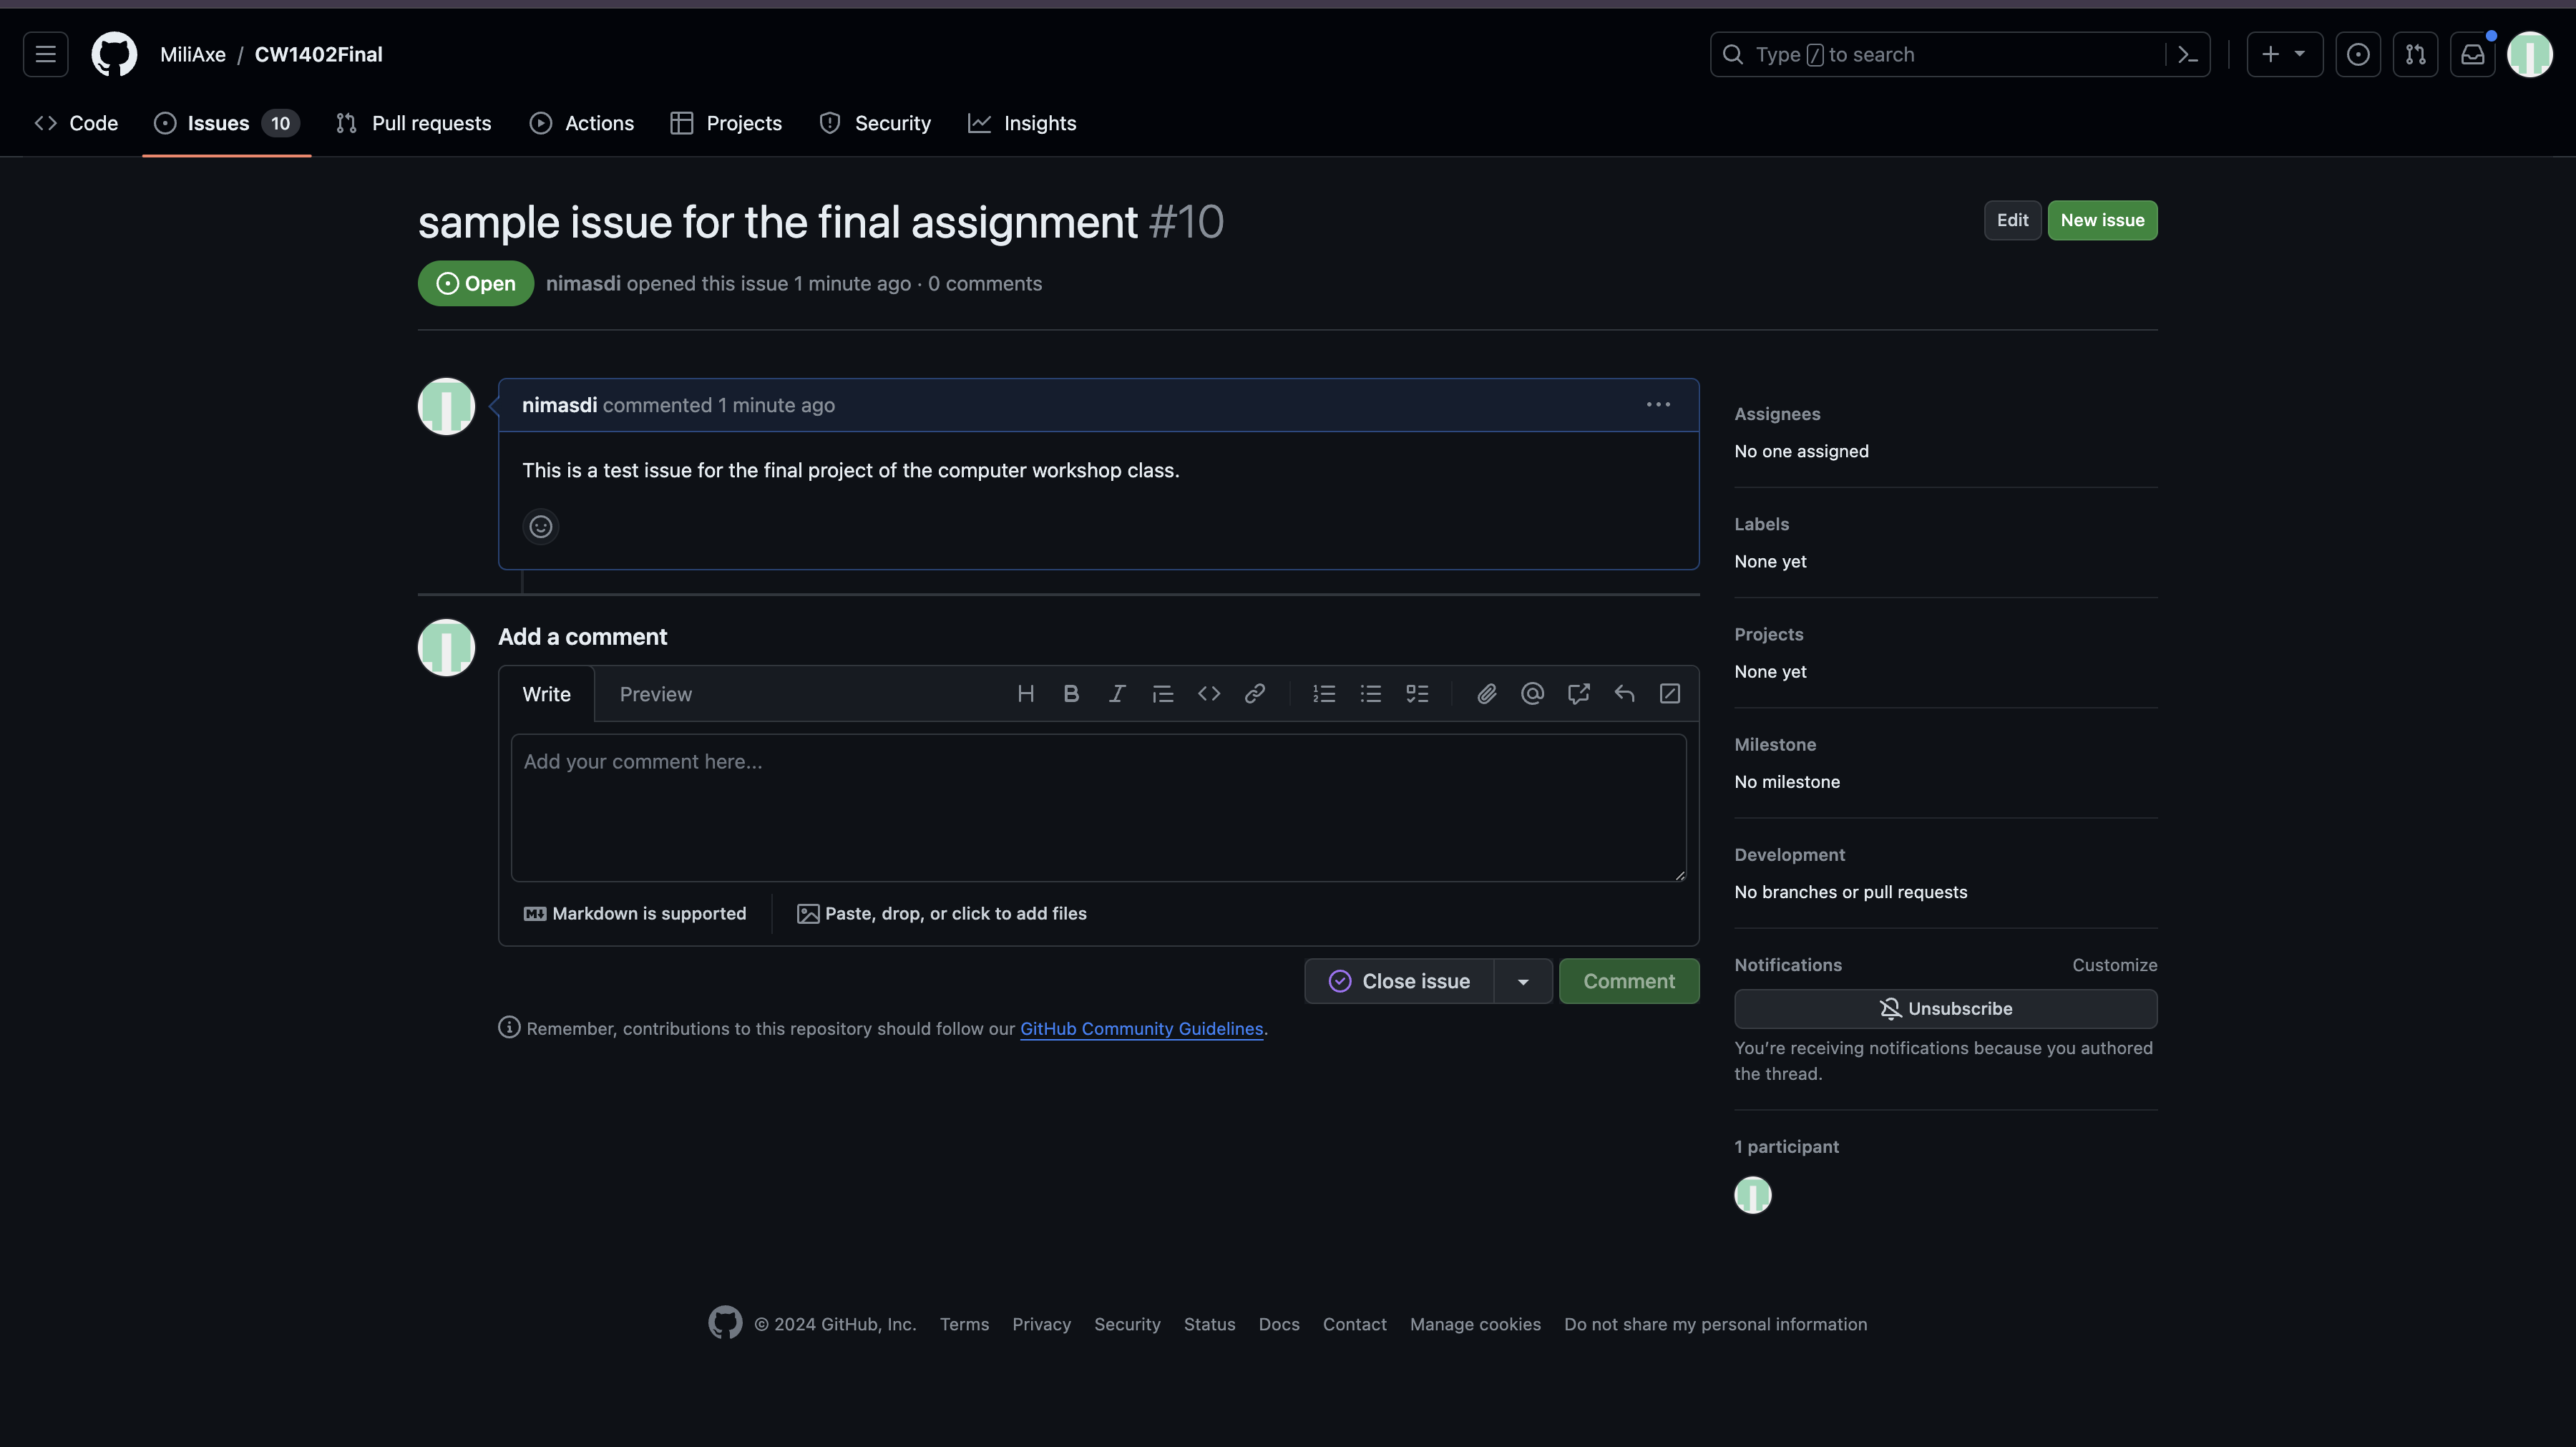
\includegraphics[width=1\textwidth]{sample-issue.png} 
\caption{The sample issue that i created}
\end{figure}


\end{document}
